% Use only LaTeX2e, calling the article.cls class and 12-point type.

\documentclass[11pt]{article}
\usepackage[round,semicolon]{natbib}
\usepackage[margin=1.4in]{geometry}
\usepackage{kpfonts}

\usepackage{seqsplit}
\usepackage{placeins}

\usepackage{newfloat}
\usepackage[labelfont=bf]{caption}
\usepackage{nameref}
\usepackage{rotating}
\usepackage{color}
\usepackage{float}

\setcounter{topnumber}{8}
\setcounter{bottomnumber}{8}
\setcounter{totalnumber}{8}
\renewcommand{\topfraction}{1}
\renewcommand{\bottomfraction}{1}
\renewcommand{\textfraction}{0}
\renewcommand{\floatpagefraction}{1}

\usepackage[font=small,labelfont=bf]{caption}

\usepackage{newfloat}
\DeclareFloatingEnvironment[name={Figure}]{suppfigure}
\renewcommand{\thesuppfigure}{S\arabic{suppfigure}}
\DeclareFloatingEnvironment[name={Table}]{supptable}
\renewcommand{\thesupptable}{S\arabic{supptable}}
\DeclareFloatingEnvironment[name={File}]{suppfile}
\renewcommand{\thesuppfile}{S\arabic{suppfile}}

\definecolor{darkblue}{rgb}{0, 0.0, 0.6}

\usepackage{hyperref}
\hypersetup{colorlinks,citecolor=blue,linkcolor=blue,urlcolor=blue}

\usepackage{seqsplit}

\usepackage{array}
\newcolumntype{R}[1]{>{\raggedright\arraybackslash}p{#1}}
\newcolumntype{C}[1]{>{\centering\let\newline\\\arraybackslash\hspace{0pt}}m{#1}}

\newcommand{\comment}[1]{{\color{red}[\textsl{#1}]}}

\usepackage{setspace}

\renewcommand{\topfraction}{1}
\renewcommand{\bottomfraction}{1}
\renewcommand{\textfraction}{0}
\renewcommand{\floatpagefraction}{1}


\title{Deep mutational scanning of an H3 hemagglutinin can inform evolutionary forecasting of human H3N2 influenza virus} 

\author{
Juhye M. Lee$^{1,4,5,\dagger}$ \and 
John Huddleston$^{2,6,\dagger}$ \and 
Michael B. Doud$^{1,4,5}$ \and 
Kathryn A. Hooper$^{1,6}$ \and
Trevor Bedford,$^{2,3}$ \and 
Jesse D. Bloom$^{1,3,4*}$
\\
\scriptsize{$^1$Basic Sciences Division, $^2$Vaccine and Infectious Diseases Division, and $^3$Computational Biology Program,} \\
\scriptsize{Fred Hutchinson Cancer Research Center, Seattle, WA, USA} \\
\scriptsize{$^4$Department of Genome Sciences, $^5$Medical Scientist Training Program, and $^6$Molecular and Cellular Biology Program,} \\
\scriptsize{University of Washington, Seattle, WA, USA} \\
\scriptsize{$^{\dagger}$These authors contributed equally} \\
\scriptsize{$^*$Correspondence: \href{jbloom@fredhutch.org}{jbloom@fredhutch.org}}
}

\date{}


\begin{document}

\maketitle
\onehalfspacing

\begin{abstract}
Abstract text.
\end{abstract}

\section*{INTRODUCTION}


\section*{RESULTS}
\label{sec:results}

\subsection*{Strategy for deep mutational scanning of an H3 hemagglutinin}

\begin{figure}
\centerline{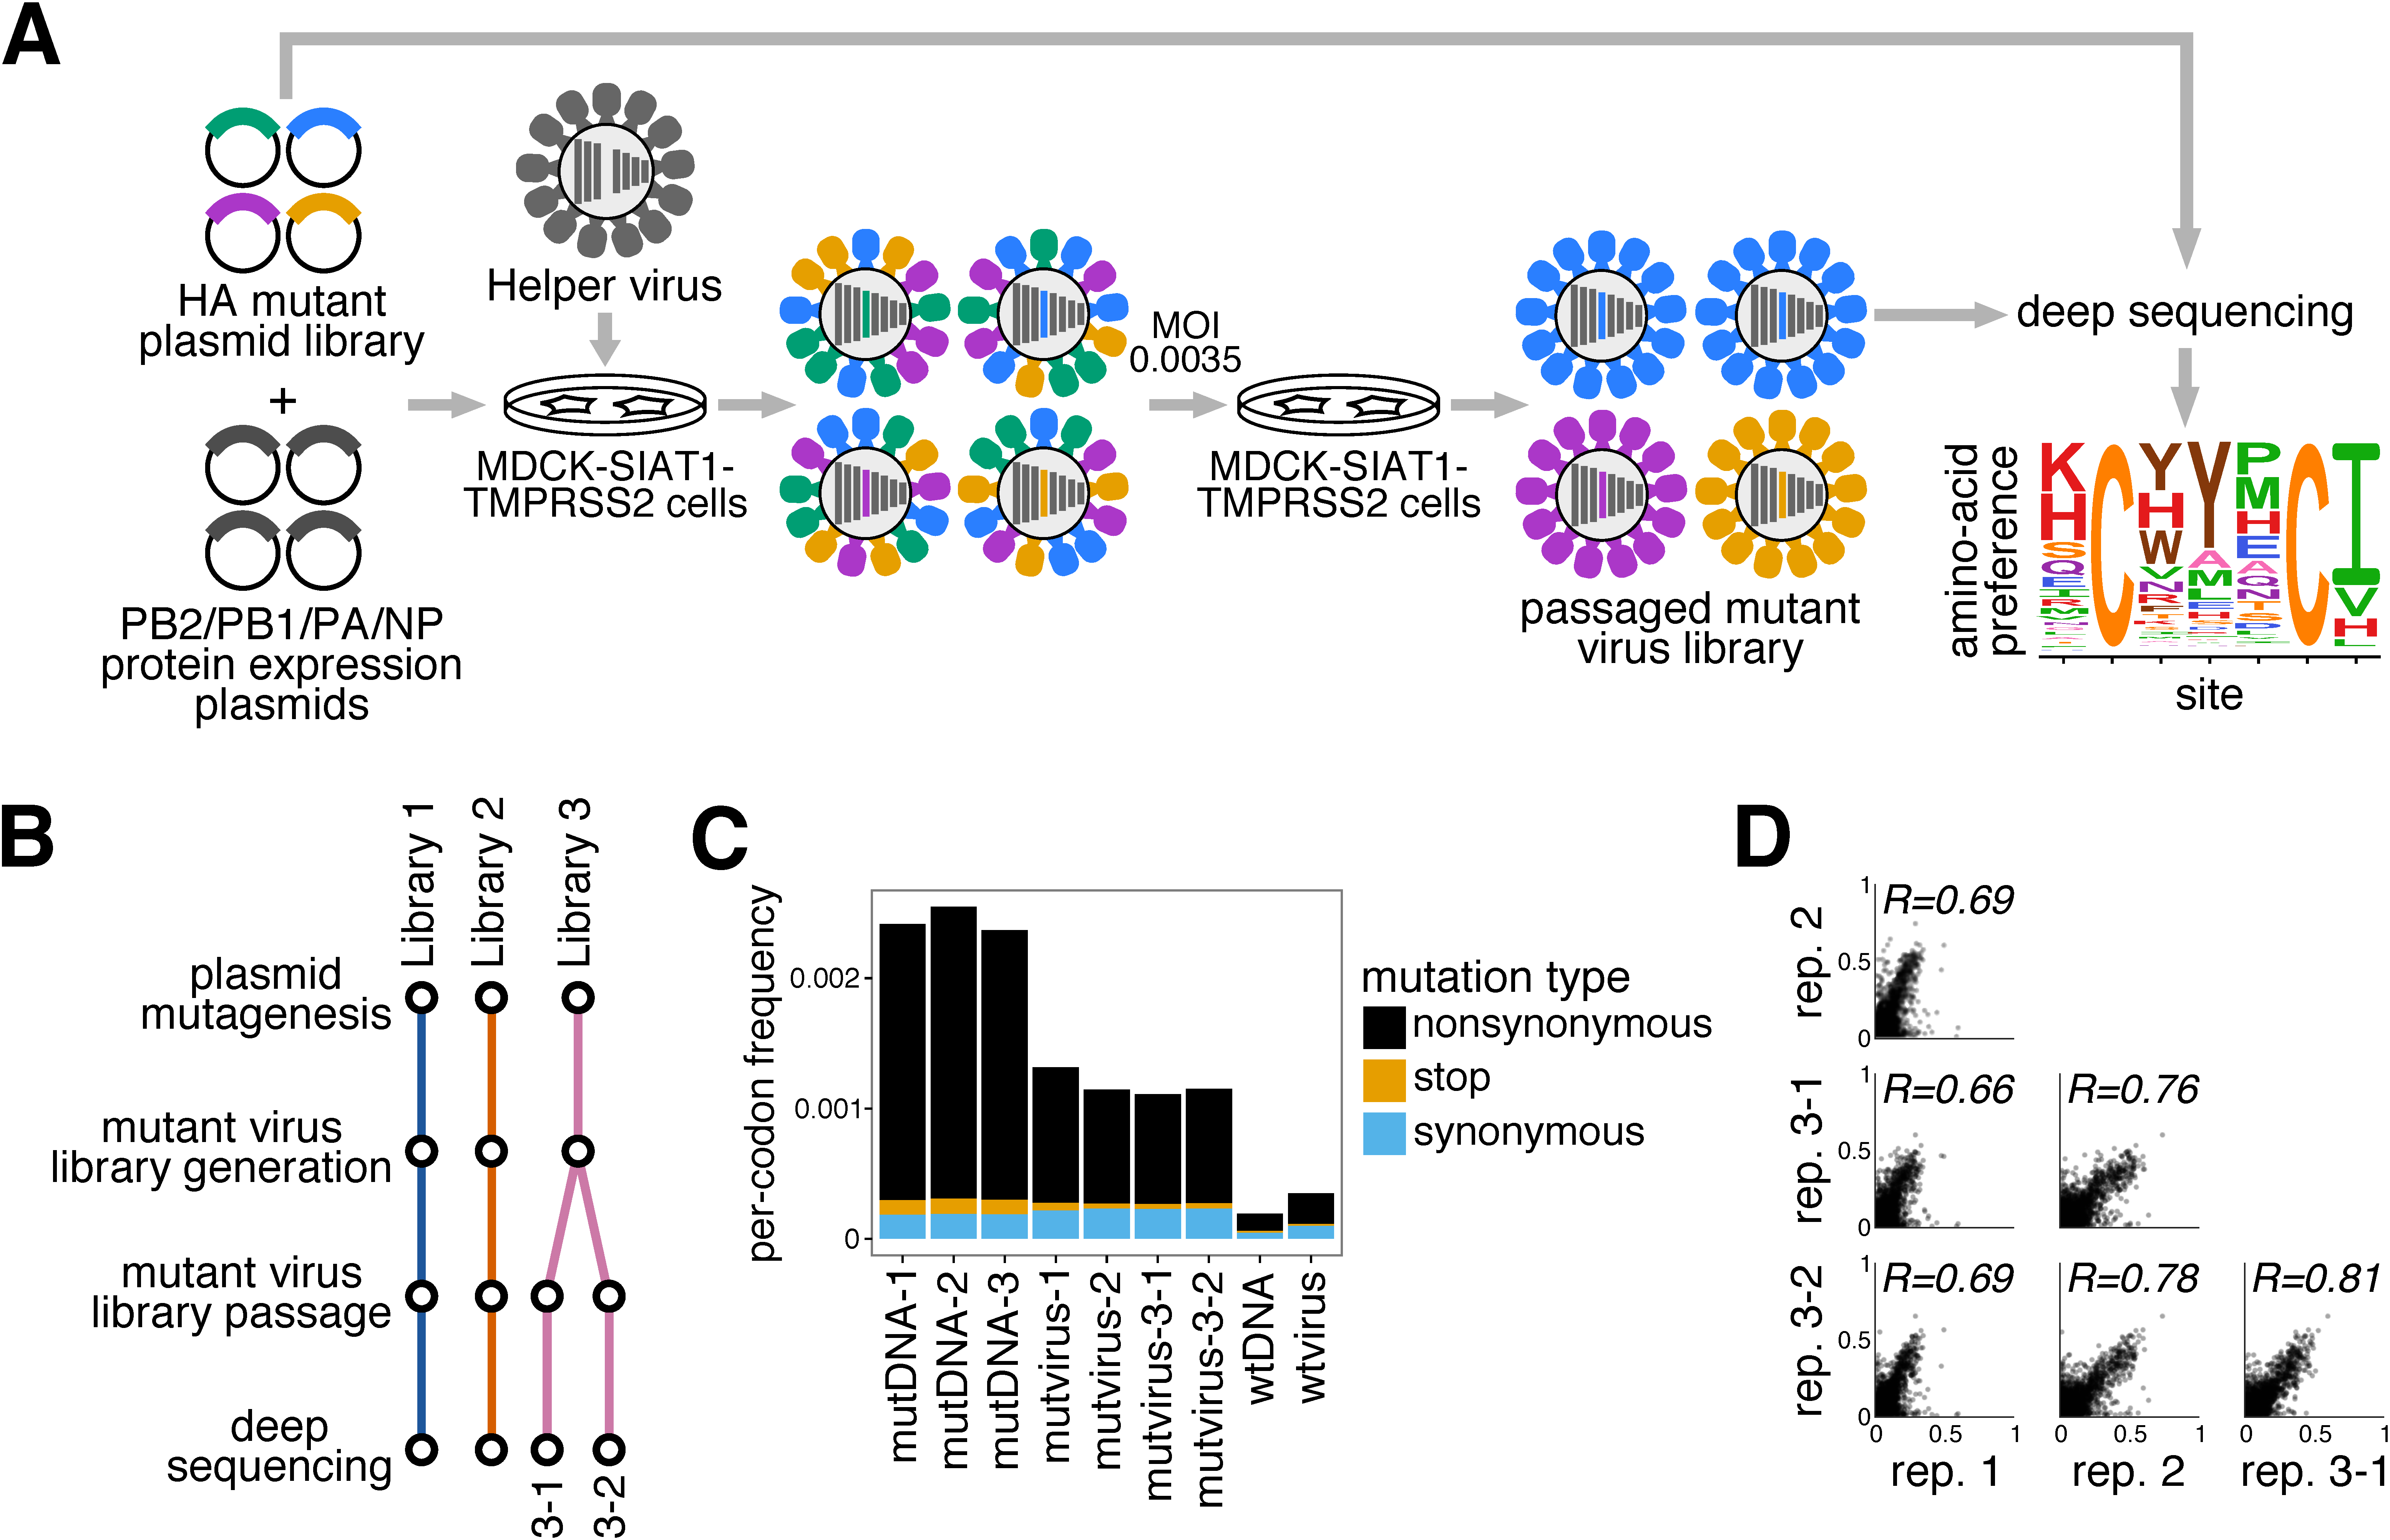
\includegraphics[width=\textwidth]{figs/dms_overview/dms_overview.pdf}}
\caption{\label{fig:dms_overview}
{\bf Overview of deep mutational scanning experiments of H3 hemagglutinin}
Figure caption text
}
\end{figure}


\subsection*{H3 site-specific amino-acid preferences}

\begin{figure}
\centerline{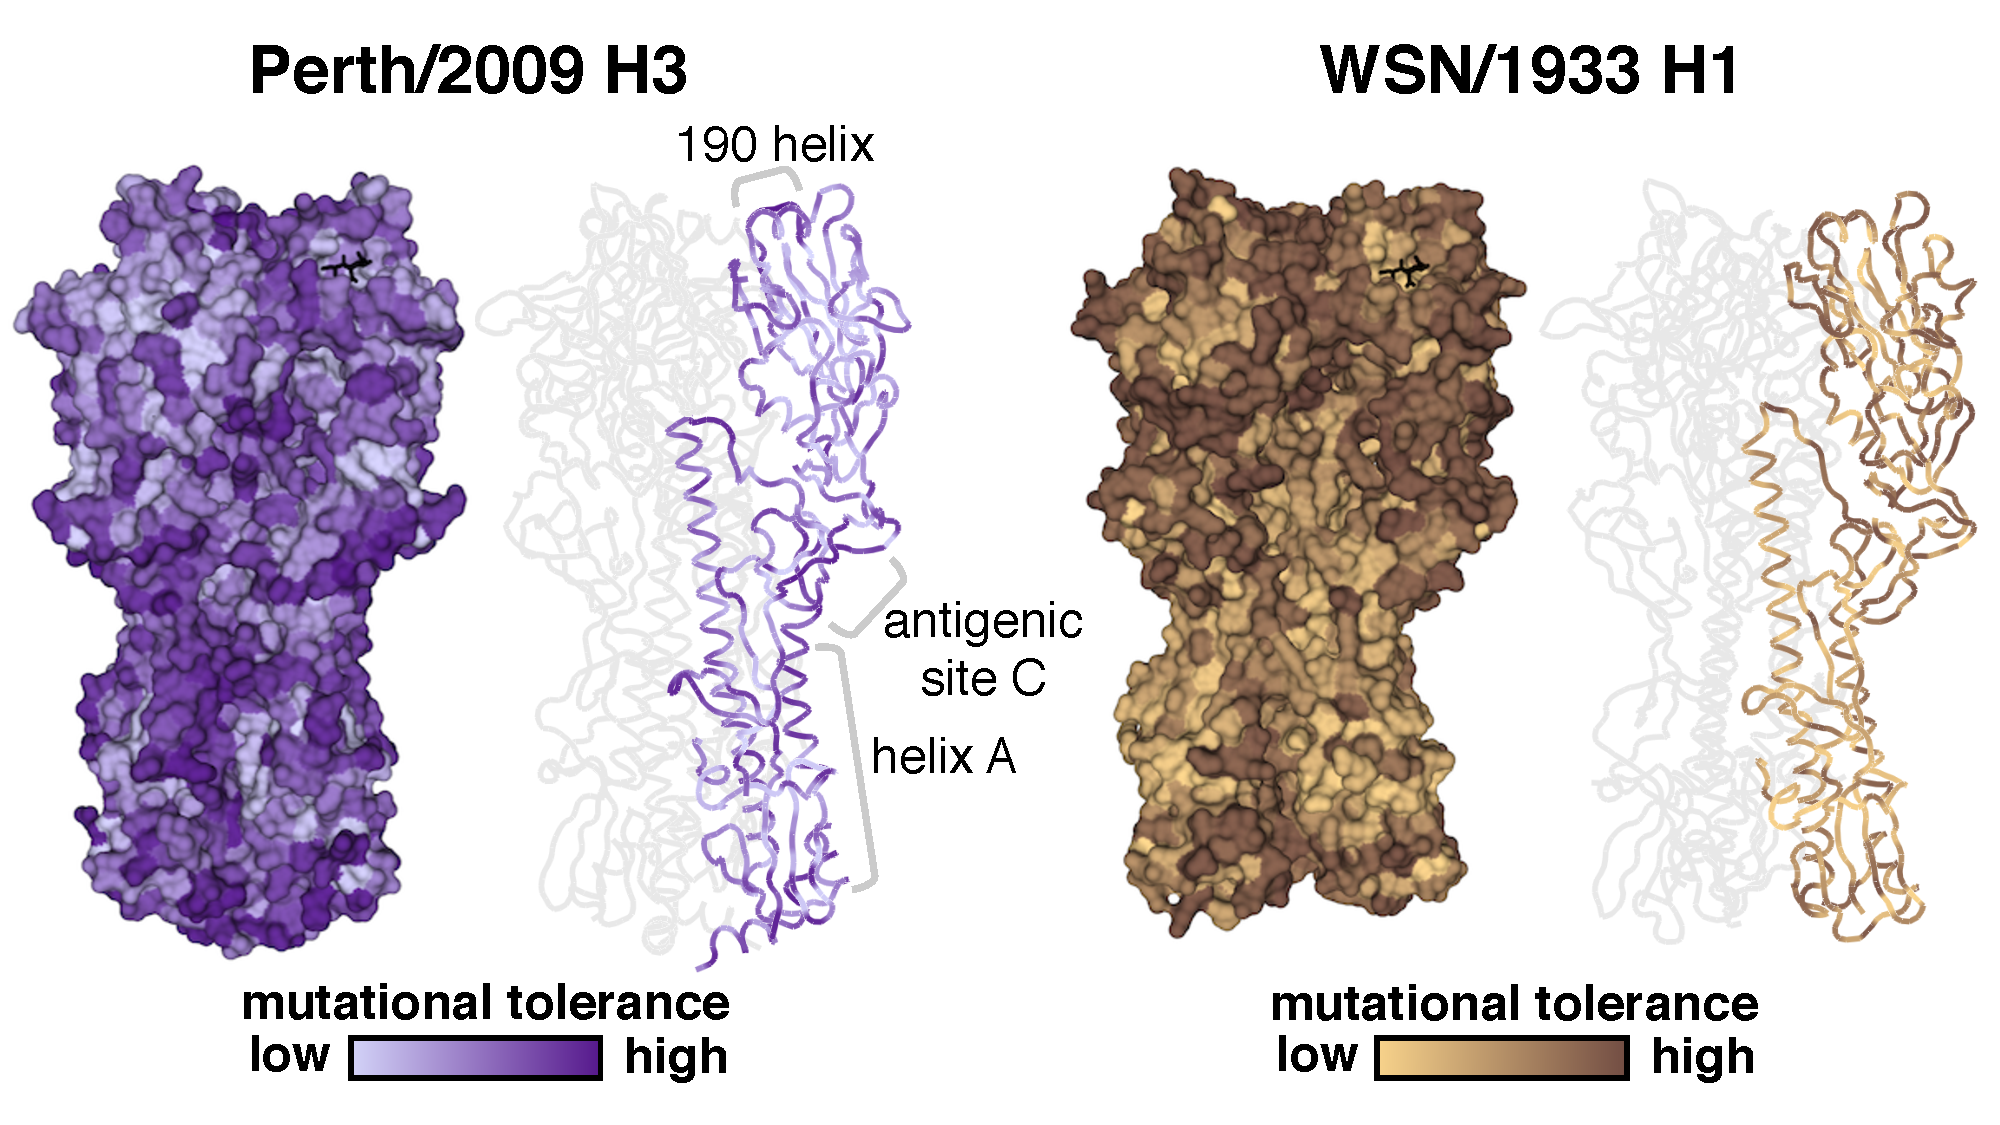
\includegraphics[width=\textwidth]{figs/mut_tolerance/entropy_heatmap.pdf}}
\caption{\label{fig:mut_tolerance}
{\bf The mutational tolerance of HA}
Figure caption text
}
\end{figure}

\begin{figure}
\centerline{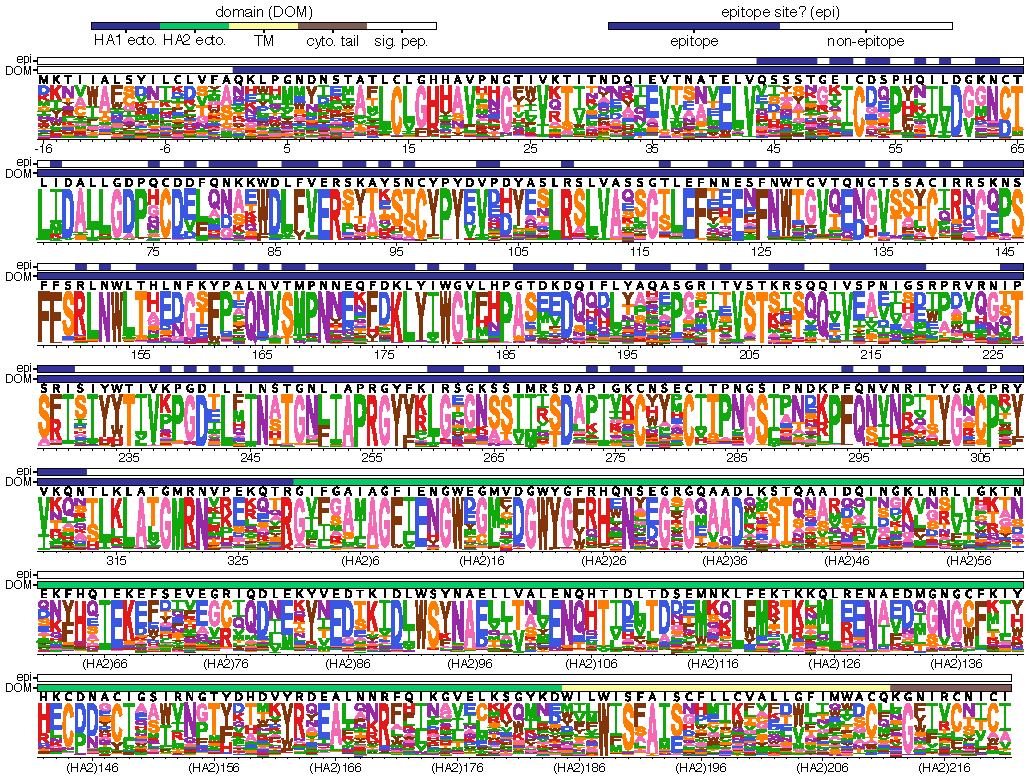
\includegraphics[width=\textwidth]{figs/prefslogoplot/rescaled-avgprefs_prefs.pdf}}
\caption{\label{fig:logoplot}
{\bf The site-specific amino-acid preferences of H3 hemagglutinin}
Figure caption text
}
\end{figure}


\subsection*{Estimating mutational effects from an H3N2 phylogeny}

\begin{figure}
\centerline{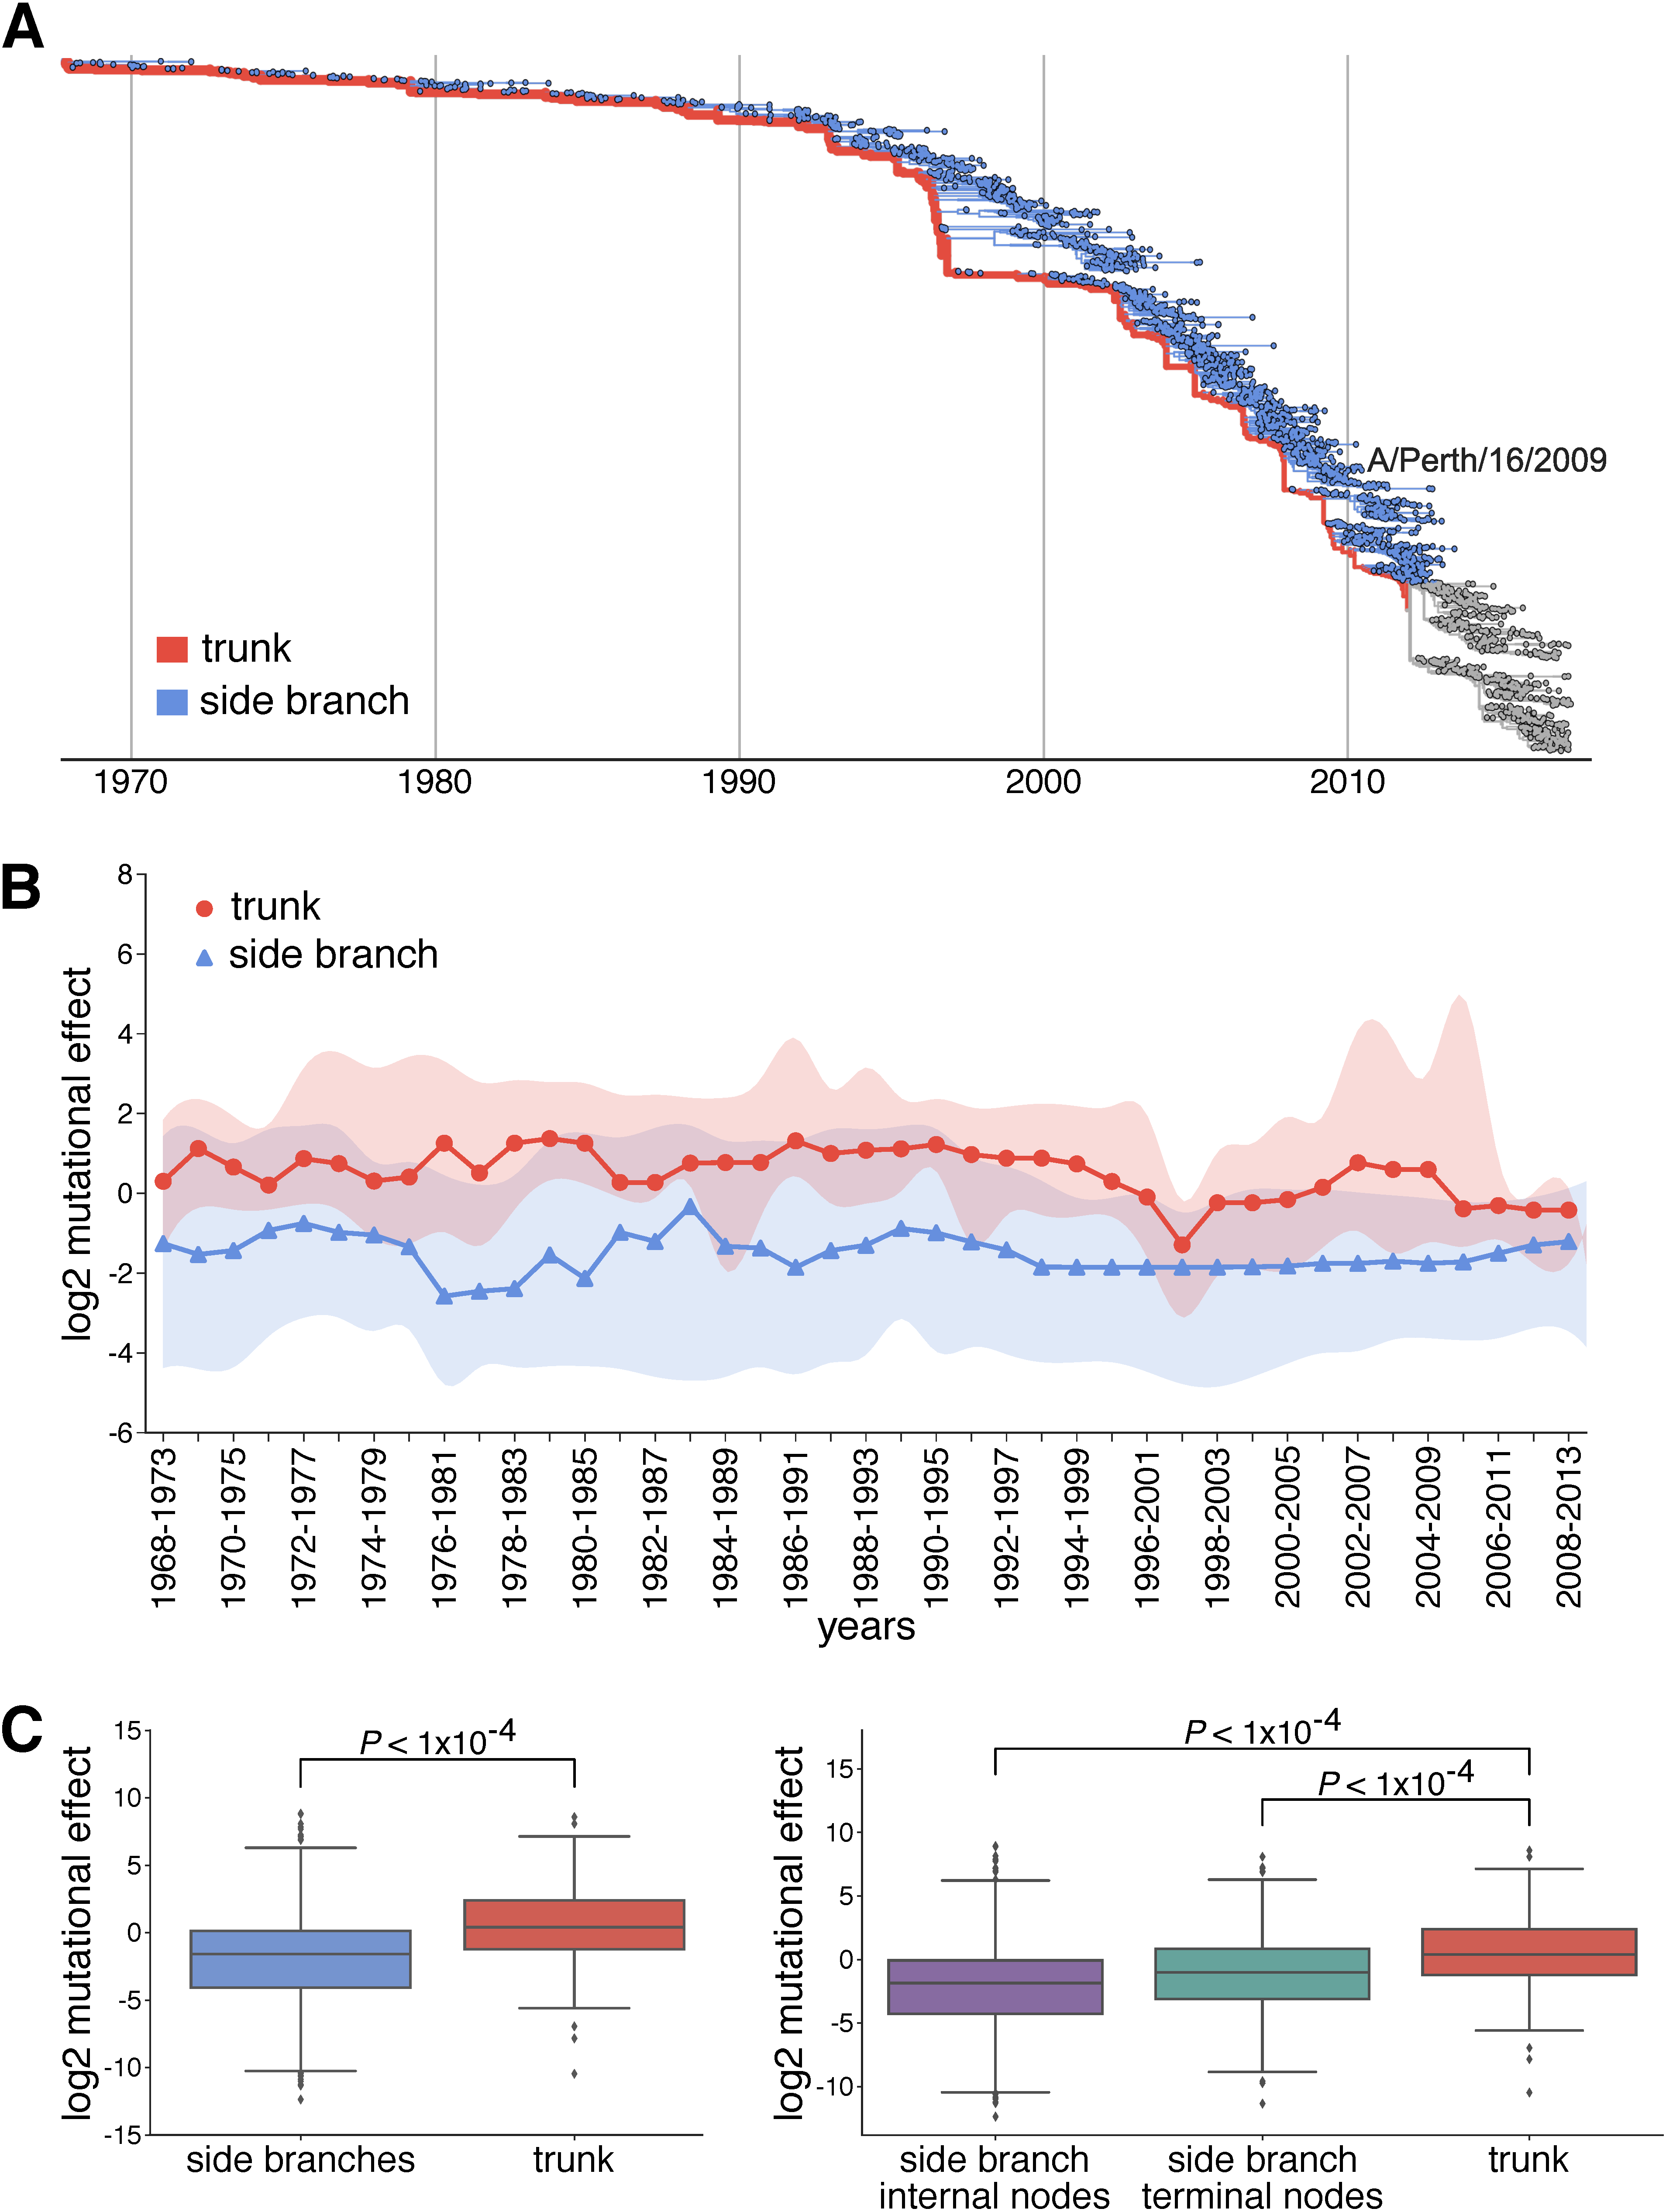
\includegraphics[width=\textwidth]{figs/trunkvssidebranch/trunkvssidebranch.pdf}}
\caption{\label{fig:trunkvssidebranch}
{\bf The trunk of a human H3N2 phylogeny has higher mutational effects than those of side branches}
Figure caption text
}
\end{figure}

\begin{figure}
\centerline{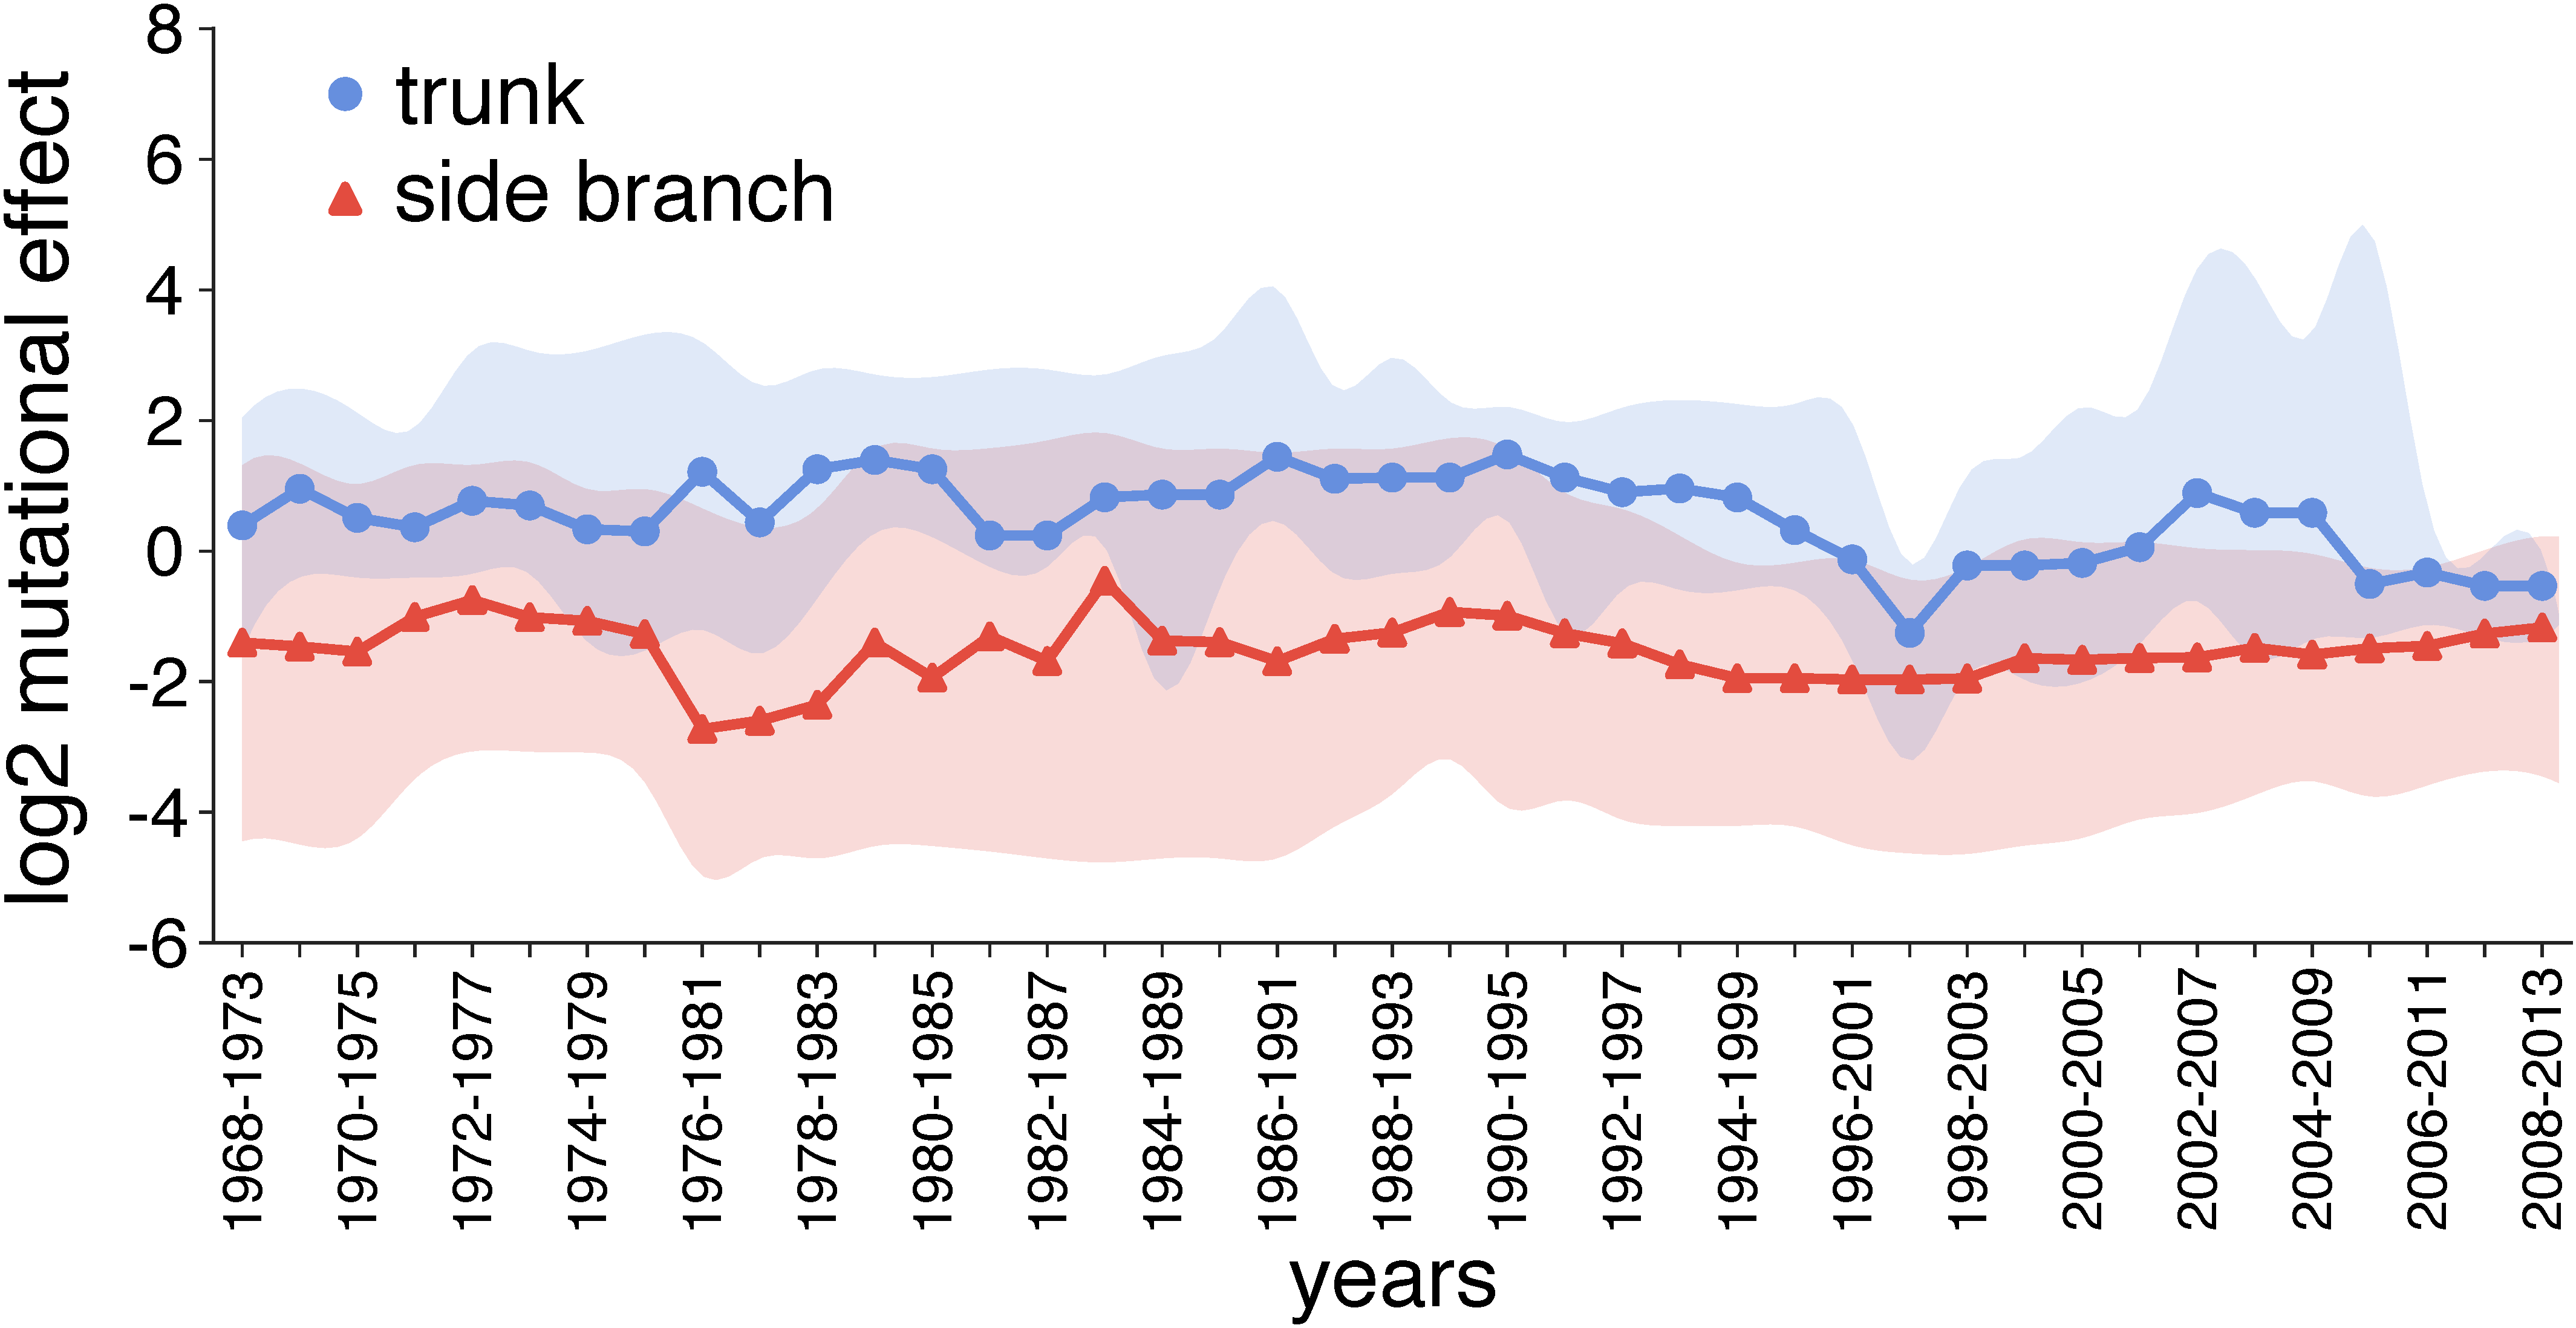
\includegraphics[width=\textwidth]{figs/muteffects_sliding_window/muteffects_sliding_window.pdf}}
\caption{\label{fig:muteffects_sliding_window}
{\bf Sliding window analysis of mutational effects of trunk vs side branches.}
Figure caption text
}
\end{figure}

\begin{figure}
\centerline{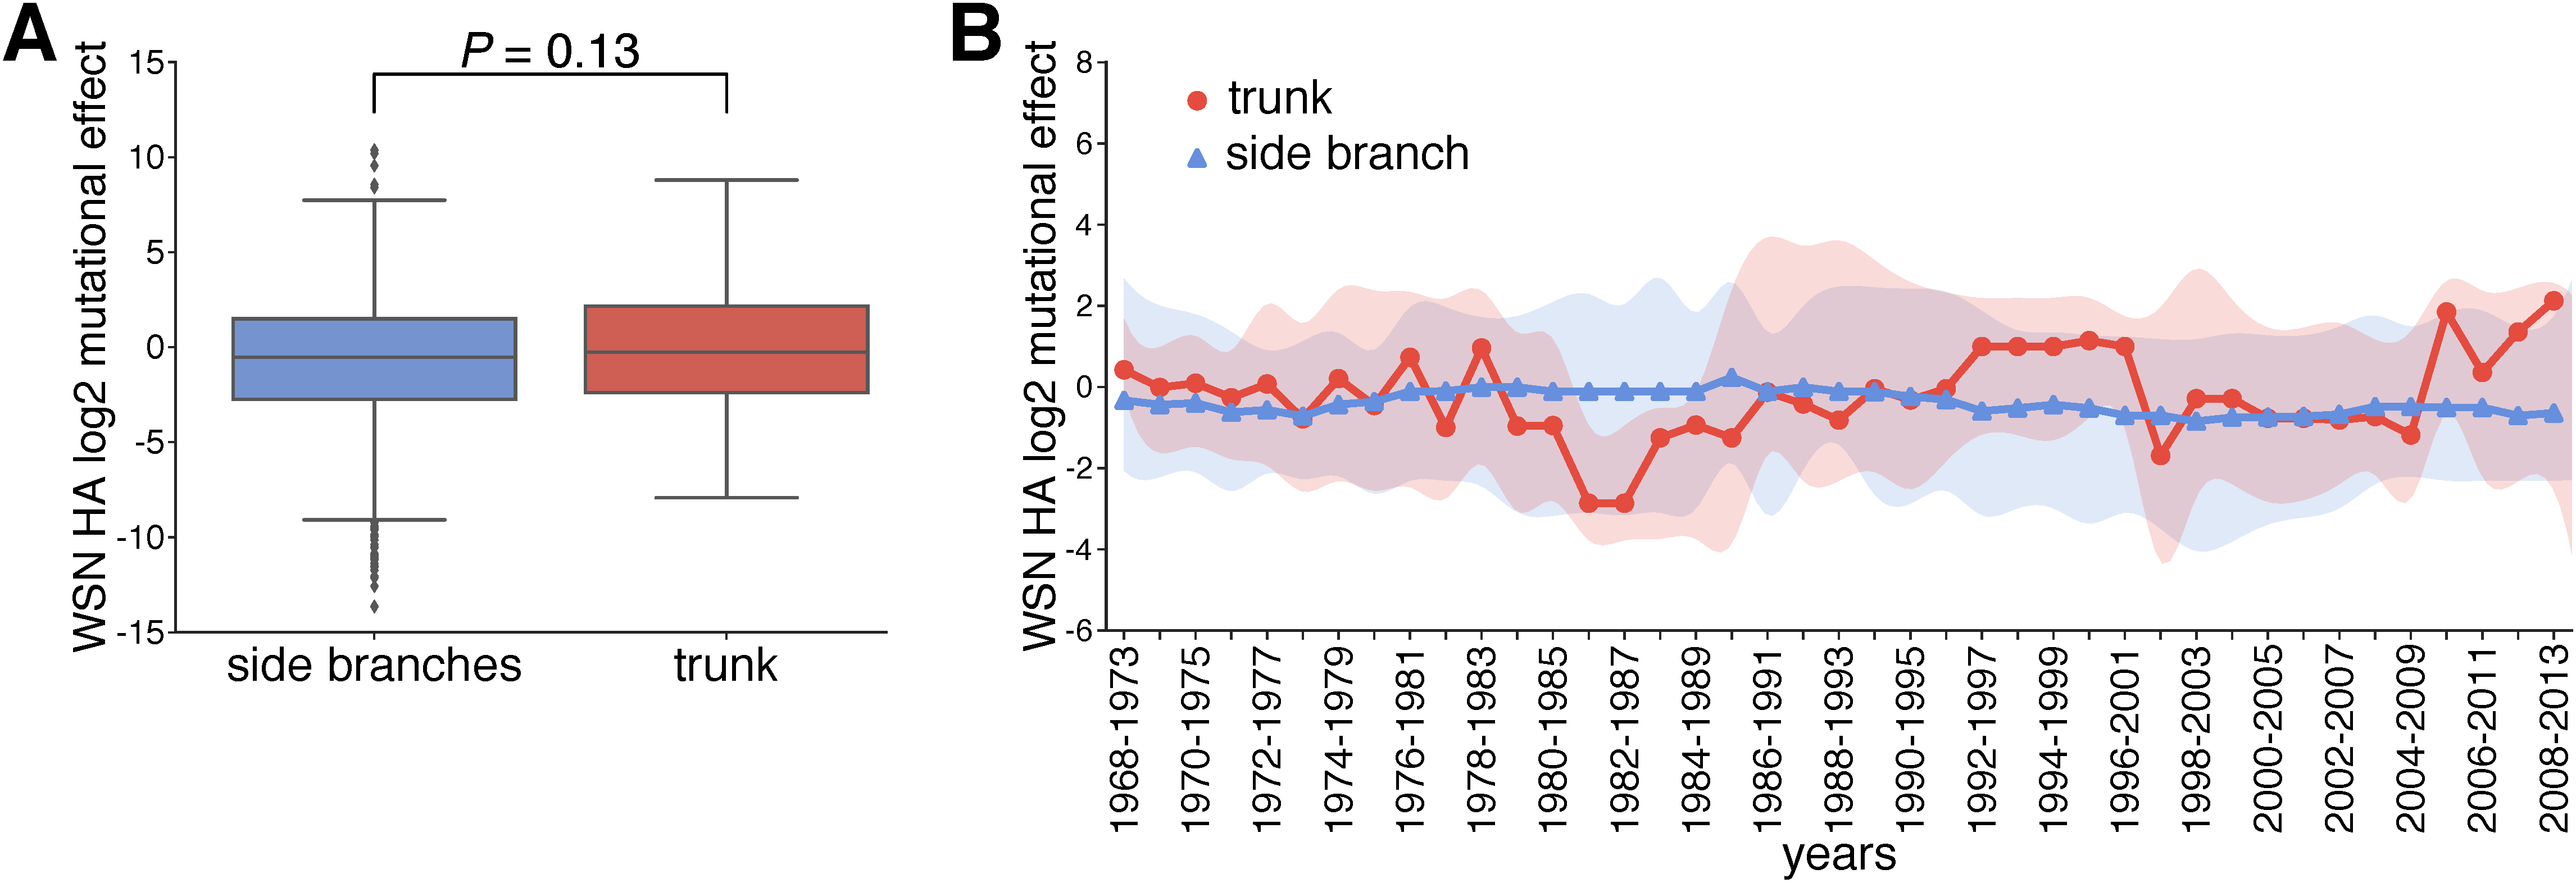
\includegraphics[width=\textwidth]{figs/WSN_trunkvssidebranch/WSN_trunkvssidebranch.pdf}}
\caption{\label{fig:WSN_trunkvssidebranch}
{\bf Trunk vs side branch mutational effects calculated using WSN preferences}
Figure caption text
}
\end{figure}


\subsection*{Comparing H1 and H3 preferences}

\begin{figure}
\centerline{\includegraphics[width=\textwidth]{figs/distance_distribution/distance_distribution.pdf}}
\caption{\label{fig:distance_distribution}
{\bf Distribution of preference shifts for protein homologs}
Figure caption text
}
\end{figure}

\begin{figure}
\centerline{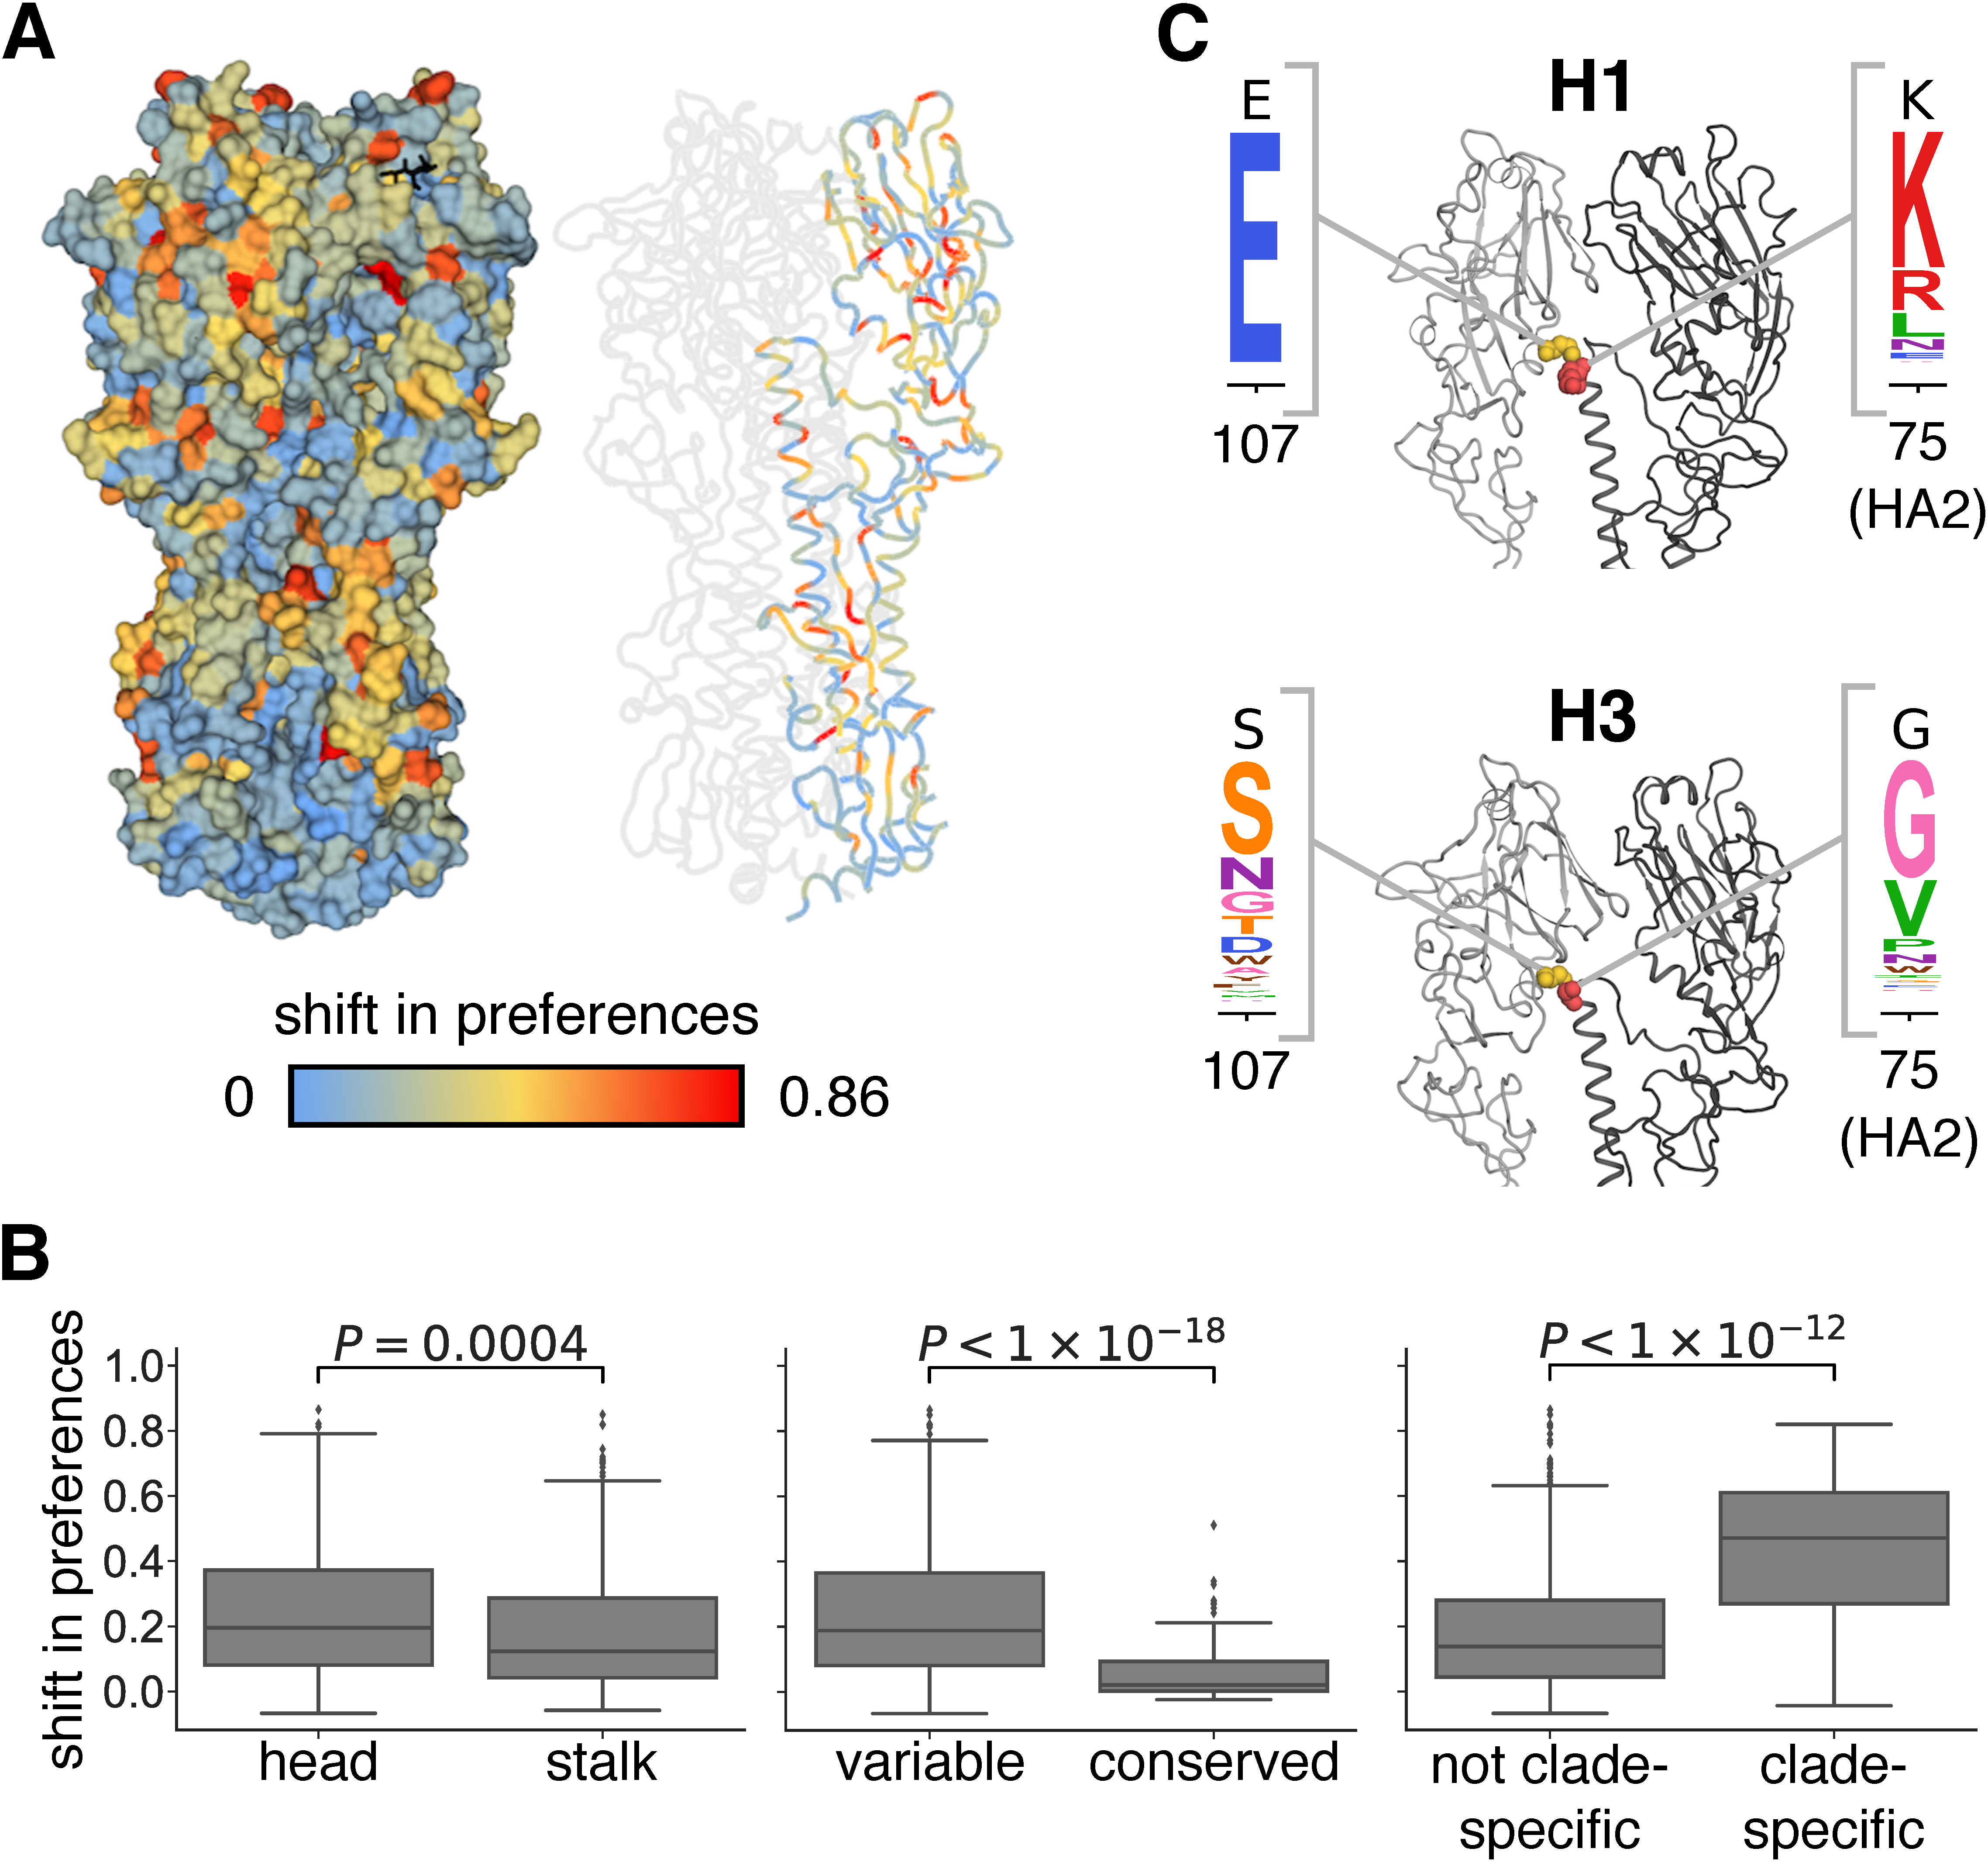
\includegraphics[width=0.5\textwidth]{figs/RMSD_heatmap/RMSD_heatmap.pdf}}
\caption{\label{fig:RMSD_heatmap}
{\bf Shifts in preferences mapped onto the structure of HA}
Figure caption text
}
\end{figure}


\section*{DISCUSSION}


\clearpage
\small

\section*{METHODS}
\label{sec:methods}
\subsection*{HA numbering}

\subsection*{Generation of HA codon mutant plasmid libraries}

\subsection*{Generation and passaging of mutant viruses}

\subsection*{Barcoded subamplicon sequencing}

\subsection*{Analysis of deep sequencing data}

\subsection*{Quantification of mutational effects and sequence preferences from an H3N2 phylogeny}

\subsection*{Data availability and source code}
Deep sequencing data are available from the Sequence Read Archive under BioSample accession \comment{add accession}.


\subsection*{ACKNOWLEDGMENTS}
We thank Sarah Hilton, Hugh Haddox...the Fred Hutch Genomics Core
Funding...


\end{document}